\documentclass[]{beamer}

\usepackage{beamerthemesplit} 
\usepackage{amsmath}
\usepackage{graphicx}
\usepackage{amsthm}
\usepackage{amssymb}
\usepackage{algorithm}
\usepackage{algpseudocode}
\usepackage{verbatim}
\usepackage{bbm}

\newcommand{\bA}{\mathbf{A}}
\newcommand{\bH}{\mathbf{H}}
\newcommand{\bX}{\mathbf{X}}
\newcommand{\bP}{\mathbf{P}}
\newcommand{\bB}{\mathbf{B}}
\newcommand{\bD}{\mathbf{D}}
\newcommand{\bS}{\mathbf{S}}
\newcommand{\bR}{\mathbf{R}}
\newcommand{\bJ}{\mathbf{J}}
\newcommand{\bV}{\mathbf{V}}
\newcommand{\bQ}{\mathbf{Q}}
\newcommand{\bLambda}{\mathbf{\Lambda}}

\title{Joint Embedding of Graphs}    % Enter your title between curly braces
\author{Shangsi Wang}                 % Enter your name between curly braces
\institute{Johns Hopkins University}      % Enter your institute name between curly braces
\date{\today}                    % Enter the date or \today between curly braces

\begin{document}

% Creates title page of slide show using above information
\begin{frame}
  \titlepage
\end{frame}
\note{Talk for 45 mins} % Add notes to yourself that will be displayed when
                           % typeset with the notes or notesonly class options

\section[Introduction]{}

% Creates table of contents slide incorporating
% all \section and \subsection commands



\begin{frame}
	\frametitle{Motivation}
	Feature extraction and dimension reduction for networks is critical in a wide variety of domains. There are a few unsupervised feature methods available: Principal Component Analysis, Graph Statistics, Graph Spectral Statistics, Laplacian Engenmap and Adjacency Spectral Embedding. We want a method which 
	\begin{itemize}
		\item Take advantage of multiple graphs,
		\item Utilize low rank property of adjacency matrix,
		\item Able to apply to sparse large graphs,
		\item Lead to good inference performance,
		\item With theoretical support. 
	\end{itemize}
	Motivate by these properties, we propose a method to jointly embed multiple undirected graphs. 
\end{frame}

\begin{frame}
	\frametitle{Random Dot Product Graph}
Let $F$ be a distribution on a set $\mathcal{X} \in \mathbb{R}^d$, and $\bX=[x_1^T,x_2^T,...,x_n^T] \in \mathcal{X}^n$. The notation is $(\bX,\bA) \sim RDPG(F)$, if
\[x_1,x_2,...,x_n \overset{i.i.d.}{\sim} F,\] 
	\[ \bA_{st}|\bX \sim Bernoulli(x_s^T x_t). \]
	Alternatively,
	\[ P(\bA|\bX) = \prod_{s<t} (x_s^T x_t) ^{ \bA_{st}} (1-x_s^T x_t)^{1- \bA_{st}}.\]
	When the latent positions $\bX$ is regarded as parameter, the notation becomes $\bA \sim RDPG(\bX)$.
\end{frame}



\begin{frame}
	\frametitle{Adjacency Spectral Embedding}
For one graph, $d$-dimensional Adjacency Spectral Embedding (ASE) approximates $\bA$ by the product of rank $d$ matrices.
\begin{equation} 
	\bA \approx \hat{\bV} \hat{\bD} \hat{\bV} ^T = \sum_{k=1}^{d} \hat{\bD}_{kk} \hat{v}_k \hat{v}_k^T  \text{ , or } \min \|\bA -\hat{\bV} \hat{\bD} \hat{\bV} \|
\end{equation}
Let the embedding $\hat{\bX}=\hat{\bV} \hat{\bD}^{\frac{1}{2}}$ which can be understand as the features of vertices or an estimator for $\bX$ under RDPG model. The distance between two embeddings,
\[d(\hat{\bX}_1,\hat{\bX}_2)= \underset{\bQ,\bQ^T\bQ=I}{\min} \|\hat{\bX}_1 \bQ- \hat{\bX}_2 \| \]
Can we embed multiple graphs together? 
\end{frame}


\section{Methodology}
\begin{frame}
	\frametitle{Multiple Random Eigen Graph}
Let $\{h_k\}_{k=1}^{d}$ be a set of norm-1 vectors in $\mathbb{R}^{n}$, and  $F$ be a distribution on a set $\mathcal{X} \in \mathbb{R}^d$. The $m$ pairs $\{(\lambda_i, \bA_i)\}_{i=1}^m$ follow a $d$-dimensional multiple random eigen graphs model, and the notation is $\{(\lambda_i,\bA_i)\}_{i=1}^m \sim MREG(F,h_1,...,h_d)$, if 
\[\{\lambda_i\}_{i=1}^m \overset{i.i.d.}{\sim} F, \]
\[ \bA_{i}[s,t]  | \lambda_i \sim Bernoulli( \sum_{k=1}^{d} \lambda_{i}[k] h_{k} [s] h_{k} [t] ). \]
In cases that $\{\lambda_i\}_{i=1}^m$ are of primary interest, 
\[\{\bA_i\}_{i=1}^{m} \sim MREG(\lambda_1,...,\lambda_m,h_1,...,h_d).\] 
\end{frame}



\begin{frame}
	\frametitle{Joint Embedding of Graphs}
Given adjacency matrices $\{A_i\}_{i=1}^m$, $d$-dimensional joint embedding of graphs is defined to be 
\begin{equation}\label{eq:1}
(\hat{\lambda}_1,...,\hat{\lambda}_m,\hat{h}_1,...,\hat{h}_d) = \underset{\lambda_i,\|h_k\|=1}{\operatorname{argmin}} \sum\limits_{i=1}^{m} \| \bA_i- \sum\limits_{k=1}^{d} \lambda_{i}[k] h_k h_k^T \|  ^2.  
\end{equation}
Here, $\hat{h}_k$ is shared across  graphs and is considered to be latent positions of vertices; $\hat{\lambda}_i$ is called loadings of graph $i$ and will be treated as features for graphs. Let $\hat{\bH}=[\hat{h}_1,...,\hat{h}_d]$ and $\hat{\bLambda}=[\hat{\lambda}_1,...,\hat{\lambda}_m]^T$.
\end{frame}


\begin{frame}
	\frametitle{Other Formulations}
	The problem can be formulated in different ways
	\begin{equation*}
	\begin{aligned}  
	& \underset{\bD_i,\|h_k\|=1}{\operatorname{argmin}} 
	& & \sum\limits_{i=1}^{m} \| \bA_i- \bH \bD_i \bH^T \|  ^2 \\
	& \text{ subject to} 
	& &  \bD_i \text{ being diagonal.}
	\end{aligned}
	\end{equation*}
	Alternatively, if $\{\bA_i\}_{i=1}^m$ are stacked in a 3-D array ${\mathbb A} \in \mathbb{R}^{m\times n \times n}$,
	\[  \underset{\bLambda,\|h_k\|=1}{\operatorname{argmin}}  \| {\mathbb A} - \sum\limits_{k=1}^{d} \bLambda_{*k} \otimes h_k \otimes h_k\|  ^2.  \]
\end{frame}

\begin{frame}
	\frametitle{Relationship to Other Factorization Methods}
	\begin{equation*}
	(\hat{\lambda}_1,...,\hat{\lambda}_m,\hat{h}_1,...,\hat{h}_d) = \underset{\lambda_i,\|h_k\|=1}{\operatorname{argmin}} \sum\limits_{i=1}^{m} \| \bA_i- \sum\limits_{k=1}^{d} \lambda_{i}[k] h_k h_k^T \|  ^2.  
	\end{equation*}
	\begin{itemize}
		\item If $h_k h_k^T$ is replaced by $\bS_k$, the problem is equivalent to principal component analysis. 
		\item If $h_k h_k^T$ is replaced by $h_k g_k^T$, the problem is equivalent to tensor rank decomposition or canonical polyadic decomposition. 
		\item If $\bD_i$ is not constrained to be diagonal and with more constrains, the problem becomes higher order SVD (Tucker Decomposition).
	\end{itemize}
\end{frame}

\begin{frame}
	\frametitle{Greedy Alternating Minimization}
We consider an algorithm which solves the problem iteratively. Specifically, at iteration $k_0$, 
\[\underset{\bLambda_{*k_0},\|h_{k_0}\|=1}{\operatorname{argmin}} \sum\limits_{i=1}^{m} \| \bA_i- \sum\limits_{k=1}^{k_0-1} \hat{\bLambda}_{ik} \hat{h}_{k} \hat{h}_{k}^T -\bLambda_{ik_0} h_{k_0} h_{k_0}^T\|  ^2.\]
Let $\bR_{ik_0} = \bA_i- \sum\limits_{k=1}^{k_0-1}\hat{\bLambda}_{ik} \hat{h}_{k} \hat{h}_{k}^T$. The gradients are, 
\begin{equation} \label{eq:3}
\frac{\partial f}{\partial h_{k_0}} = -4\sum\limits_{i=1}^{m}  \bLambda_{ik_0} (\bR_{ik}-\bLambda_{ik_0} h_{k_0} h_{k_0}^T)  h_{k_0}.
\end{equation}

\begin{equation}  \label{eq:4}
\hat{\bLambda}_{i k_0} = \langle \bR_{ik}, h_{k_0} h_{k_0}^T \rangle,
\end{equation}
\end{frame}

\begin{frame}
\frametitle{Optimization Algorithm}
\vspace{-0.2cm}
	\begin{algorithmic}[1]
		\Procedure{Find joint embedding $\hat{\bLambda},\hat{\bH}$ of $\{\bA_i\}_{i=1}^m$}{}
		\State Set residuals: $\bR_{i1}=\bA_i$
		\For{$k=1:d$ }
		\State Initialize $h_k$ and $\bLambda_{*k}$ 
		\While{not convergent}
		\State Fixing $\bLambda_{*k}$, update $h_k$ by gradient descent \eqref{eq:3}
		\State Project $h_k$ back to the unit sphere
		\State Fixing $h_k$, update $\bLambda_{*k}$ by \eqref{eq:4}
		\State Compute objective $\sum\limits_{i=1}^{m} \| \bR_{ik}-  \bLambda_{ik} h_k h_k^T \|^2$
		\EndWhile
		\State Update residuals: $\bR_{i(k+1)}=\bR_{ik}- \bLambda_{ik} h_kh_k^T$
		\EndFor
		\State Output $\hat{\bLambda}=[\bLambda_{*1},...,\bLambda_{*d}]$ and $\hat{\bH}=[h_1,...,h_d]$
		\EndProcedure
	\end{algorithmic}
\end{frame}


\begin{frame}
  \frametitle{Theory}
  \begin{theorem}
  	Given any distribution $\mathcal{F}$ on binary graphs and a random adjacency matrix $\bA \sim \mathcal{F}$, there exists a dimension  $d$, a distribution $F$ on $\mathbb{R}^d$, and a set of vectors $\{h_k\}_{k=1}^d$, such that $\bA \sim MREG(F,h_1,...,h_d)$.
  	\label{thm:rep}
  \end{theorem}
  \begin{figure}[!htbp]
  	\centering
  	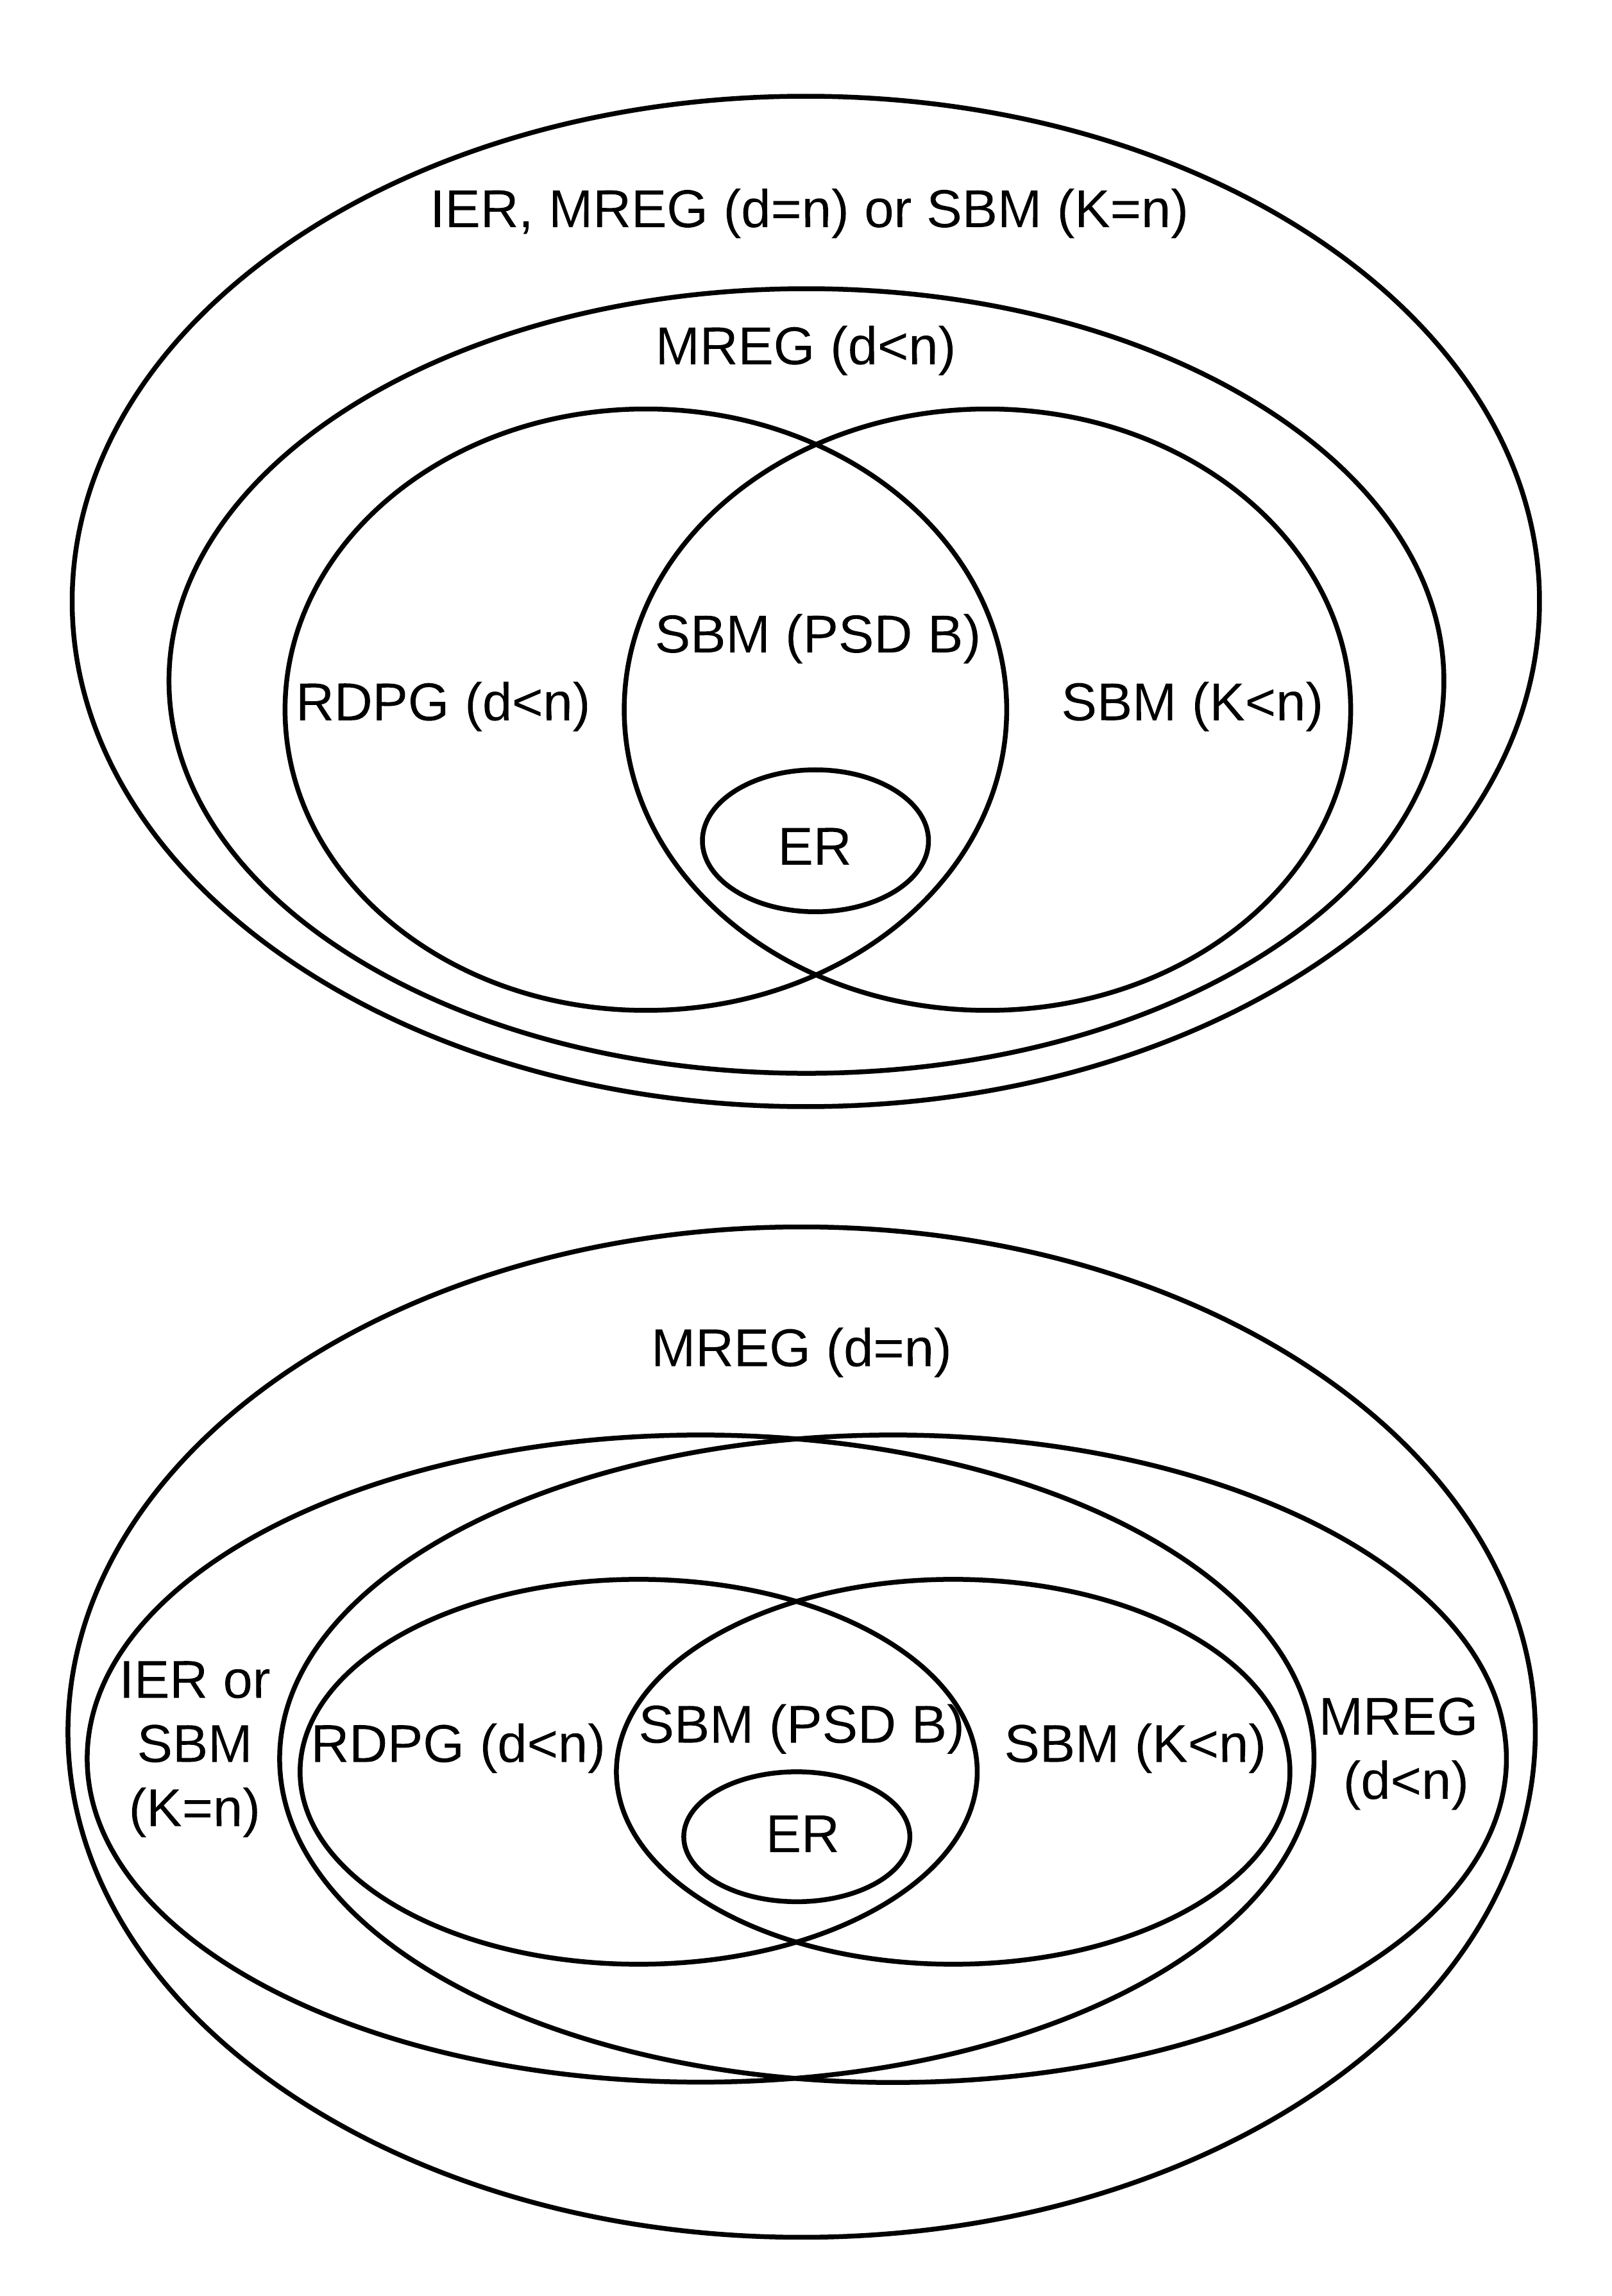
\includegraphics[scale=0.3]{ven_diag.png}
  	\caption{$\Lambda_i$ of jointly embedded graphs}
  \end{figure}
\end{frame}

\begin{frame}
	\frametitle{Theory}
	Let $\rho(\bA_i,h)= \|\bA_i- \langle \bA_i,h h^T \rangle h h^T\|^2$ and $D(h,h_1) = E(\rho(\bA_i,h))$. Under $1$-dimensional MREG model, we can show
\begin{theorem}
	\label{thm:1}
	If $D(h,h_1)$ has a unique global minimum at $h'$, then $\hat{h}_1^m$ converges almost surely to $h'$ as $m$ goes to infinity. That is, 
	\[ \hat{h}_1^m \overset{p}{\rightarrow} h'. \]
\end{theorem}

\begin{theorem}
	\label{thm:2}
	If $h'$ is a minimizer of $D(h,h_1)$, then 
	\[\|h'-h_1\| \leq \frac{2 E(\lambda_i)}{E(\lambda_i^2)(h_1^T h')^2}. \]
\end{theorem}

\end{frame}


\section{Numerical Experiments}
\begin{frame}
\frametitle{Experiment 1: Setup}
We generate 200 graphs from $2$ dimensional MREG $(\lambda_i,\bA_i)\}_{i=1}^{200} \sim MREG(F,h_1,h_2)$. The generating scheme is equivalent to the following stochastic black model, let $Y_i$ indicator for the class membership.
\[ A_i|Y_i=0 \sim  SBM((1,...,1,2,...,2),\begin{bmatrix} 0.3 & 0.2 \\ 0.2 & 0.3 \\ \end{bmatrix})  \]
\[ A_i|Y_i=1 \sim  SBM((1,...,1,2,...,2),\begin{bmatrix} 0.25 & 0.2 \\ 0.2 & 0.25 \\ \end{bmatrix})\]
These graphs are jointly embedded and classified by applying 1-Nearest Neighbor on $\hat{\lambda}_{i}$. 
\end{frame}

\begin{frame}
\frametitle{Experiment 1: Result}
We compare joint embedding to extract features to five other feature extraction approaches: Adjacency Spectral Embedding, Laplacian Eigenmap, Graph Statistics, Graph Spectral Statistics, and PCA.
\begin{figure}[!htbp]
	\centering
	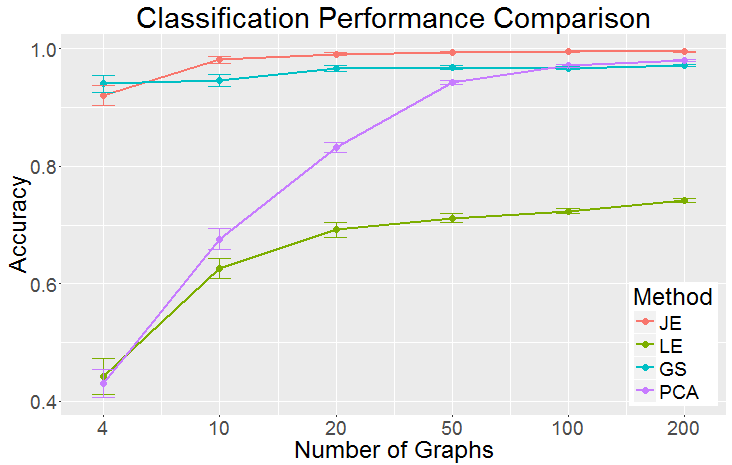
\includegraphics[scale=0.6,width=3.0in]{leig_je_acc.png}
\end{figure} 

\end{frame}

\begin{frame}
\frametitle{Experiment 2: Predict CCI}
Functional magnetic resonance images of 113 subjects are collected and converted to graphs. A covariate named creativity index is also measured for each subject. We try to predict creativity index based on the neural connectivity. We first jointly embed 113 graphs, then regress creativity index on $\hat{\lambda}_{i}$,
\[CCI_i \sim \beta_0+\hat{\lambda}_i^T\beta + \epsilon_i. \]
The p-value compared to null model is around $0.0018$.
\end{frame}


\begin{frame}
	\frametitle{Experiment 2: Result}
	\begin{figure}[!htbp]
		\centering
		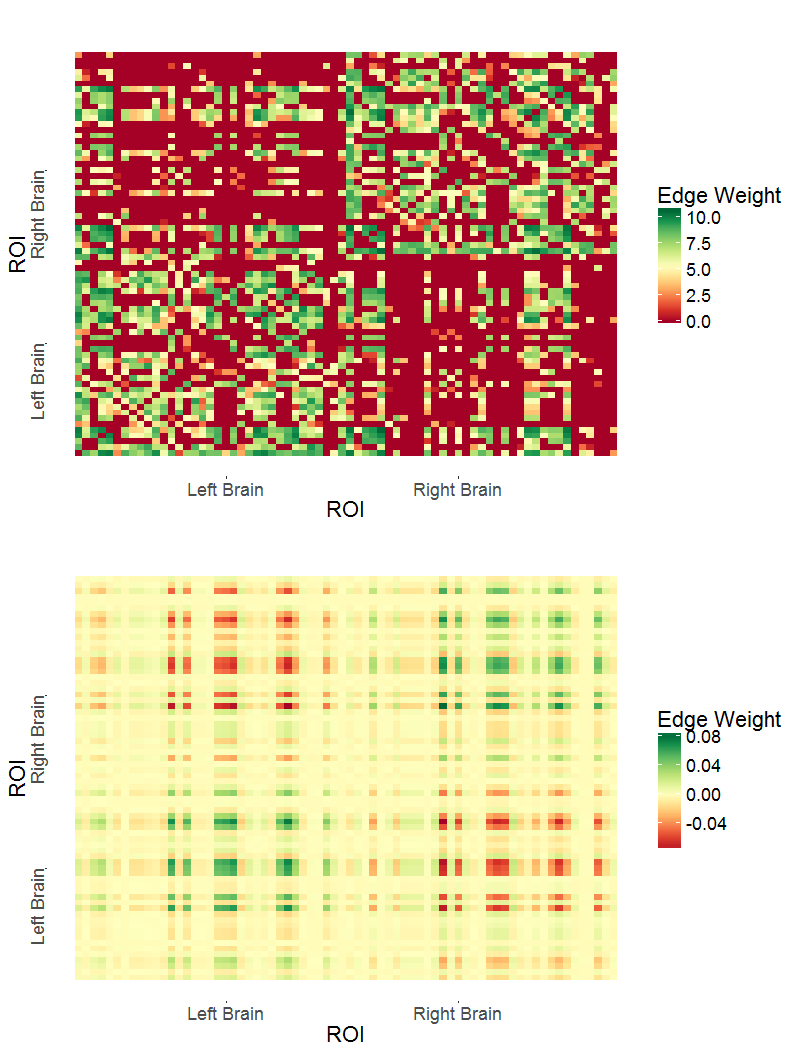
\includegraphics[scale=0.15]{cci_data.png}
		\caption{A typical brain graph and $\hat{h}_6 \hat{h}_6^T$.}
	\end{figure}
\end{frame}


\begin{frame}
	\frametitle{Experiment 2: Result}
\begin{figure}[!htbp]
	\centering
	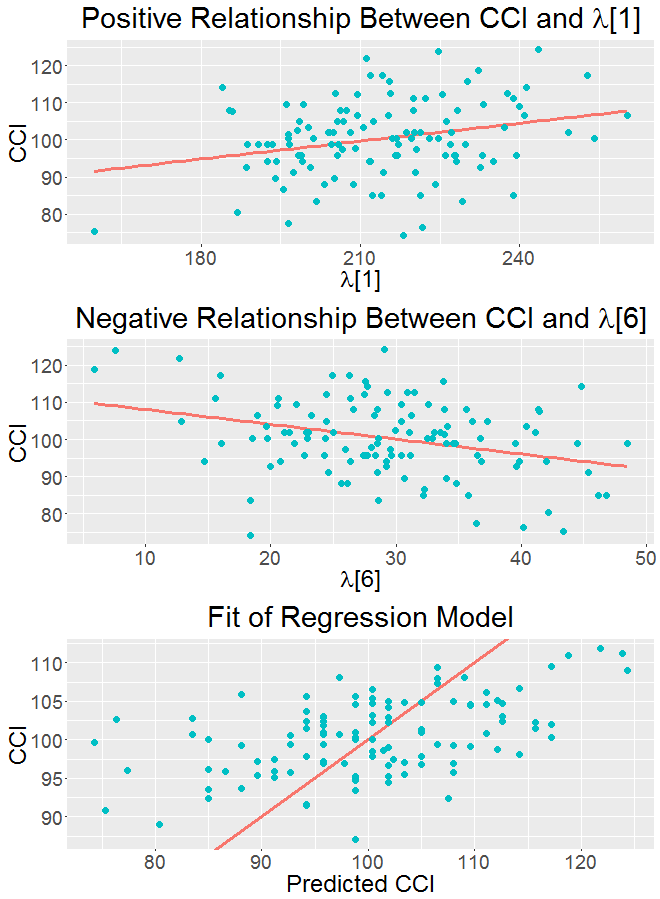
\includegraphics[scale=0.18]{cci.png}
	\caption{The relationship between CCI and $\hat{\lambda}$.}
	\label{fig:cci}
\end{figure}
\end{frame}

\begin{frame}
	\frametitle{Experiment 3: Clustering Wikipedia Pages}
	We apply the spectral clustering approach to Wikipedia graphs. The vertices of these graphs represent Wikipedia article pages. The two vertices are connected by an edge if either of the associated pages hyperlinks to the other. Two graphs are constructed based on English webpages and French webpages.We consider a subset vertices  from $3$ categories: People, Things, Math Terms.
	\begin{table}[]
		\centering
		\begin{tabular}{|l|l|l|l|l|}
			\hline
			Method& ASE+EN  & ASE+FR  & JE+EN & JE+FR \\\hline
			ARI& 0.147 & 0.115  &{\bf 0.158} & 0.156   \\\hline
			Purity& 0.549 & 0.520 &{\bf 0.551} & 0.549 \\
			\hline
		\end{tabular}
		\caption{Clustering Performance on Wikipedia Graphs.}
		\label{tb:wiki}
	\end{table}
\end{frame}

\begin{frame}
	\frametitle{Experiment 3: Result}
\begin{figure}[!htbp]
	\centering
	\includegraphics[height=2.2in,width=3.0in]{latent_pos.png}
	\caption{The latent positions of English Graph estimated by the joint embedding are shown. }
	\label{fig:lp}
\end{figure}
\end{frame}



\section{Discussion}
\begin{frame}
\frametitle{Variations}
\begin{equation*}
(\hat{\lambda}_1,...,\hat{\lambda}_m,\hat{h}_1,...,\hat{h}_d) = \underset{\lambda_i,\|h_k\|=1}{\operatorname{argmin}} \sum\limits_{i=1}^{m} \| \bA_i- \sum\limits_{k=1}^{d} \lambda_{i}[k] h_k h_k^T \|  ^2.  
\end{equation*}
\begin{itemize}
	\item Constrain $\lambda_i$ to be the same within the group.
	\item Constrain $\lambda_i$ to be non-negative.
	\item Add penalty on $\lambda_i$.
	\item Use logistic loss.
	\item Include matrix such as $h_k h_{k'}^T$.
\end{itemize}
\end{frame}


\begin{frame}
\frametitle{}
{\Large This is joint work with Joshua T. Volgelstein and Carey E. Priebe.}
\newline
\newline
{\Large Thank you! Questions?}
\end{frame}


\end{document}
